\documentclass{beamer}
\mode<presentation>
{
  \usetheme{ldv}
  \setbeamercovered{transparent}
}

\newcommand{\slidenomenclature}{Slide}
\renewcommand{\contentsname}{Contents}
\renewcommand{\figurename}{Figure}
\renewcommand{\tablename}{Table}

% \usepackage[utf8]{inputenc}
% \usepackage{luatexja}
\usepackage{fontspec}
\usepackage{luatexja-fontspec}

\setmainjfont{FandolSong-Regular}

\usepackage{amsmath,amssymb,amsfonts}
\usepackage{graphicx}
\usepackage{fancyvrb}
\usepackage{array}
\usepackage{colortbl}
\usepackage{tabularx}
\usepackage{booktabs}

% Uncomment me when you need to insert code
\usepackage{color}
\usepackage{listings}
% End Code

% Uncomment me when you need video or sound
\usepackage{multimedia}
\usepackage{hyperref}
% End video
\usepackage{graphicx}
\usepackage{tikz}
\usetikzlibrary{arrows.meta, positioning}
\usetikzlibrary{calc}
\definecolor{HCMUSBlue}{HTML}{1E5CB3}

\newcommand{\coverphoto}{ldvtheme/truong.png}

\newcommand{\titlebg}{
\begin{tikzpicture}[remember picture,overlay]
    \begin{scope}
        \clip
        ($(current page.south west)+(0,0.33cm)$) --
        ($(current page.south east)+(0,0.33cm)$) --
        ($(current page.south east)+(0,9cm)$) --
        ($(current page.south west)+(0,9cm)$) -- cycle;

        \node[anchor=south west, inner sep=0, opacity=0.24]
        at (current page.south west)
        {\includegraphics[width=\paperwidth,height=8.64cm]{\coverphoto}};
    \end{scope}

    \draw[HCMUSBlue, line width=0.45pt]
    ([yshift=-0.98cm]current page.north west) --
    ([yshift=-0.98cm]current page.north east);
\end{tikzpicture}
}

\setbeamercolor{title}{fg=HCMUSBlue}
\setbeamercolor{frametitle}{fg=HCMUSBlue}

% Header
\newcommand{\zwischentitel}{Speech-to-Speech Translation for Travelers}
\newcommand{\leitthema}{CSC15012 --- Applications of NLP in Industry}
% End Header

% Titlepage
\title{\Large \textbf{SPEECH-TO-SPEECH TRANSLATION\\FOR INTERNATIONAL TRAVELERS}}
\author{%
  Tran Ly Nhat Hao \and
  Nguyen Ngoc Canh
}
\newcommand{\vndate}{\number\day/\number\month/\number\year}
\date{\vndate}
\newcommand{\presdatum}{\number\day/\number\month/\number\year}
\institute
{
  \textbf{CSC15012 --- Applications of NLP in Industry}\\
  VNUHCM --- University of Science
}
% End Titlepage


% Slides
\begin{document}

% ============================================================
% Slide 1: Title page
% ============================================================
{
\usebackgroundtemplate{\titlebg}
\begin{frame}
    \vspace*{0.4cm}
	\titlepage
\end{frame}
}


% ============================================================
% Slide 2: Business Problem Definition
% ============================================================
\begin{frame}[t]{Business Problem Definition: Context \& Motivation}
    \begin{block}{Business Context}
        As international tourism rebounds, travelers face significant friction due to language barriers in high-paced environments (e.g., ordering food, medical emergencies).
    \end{block}

    \only<2>{
        \begin{itemize}
            \item \textbf{The Problem:} There are not many translation apps specifically designed for travelers. Traditional translation apps all require users to interact with on-screen buttons during the translation process, which is slow, intrusive, and unnatural during face-to-face interactions.
            \item \textbf{Core Objective:} To provide a hands-free, low-latency bridge for travelers navigating foreign-language environments (e.g., US, Japan).
        \end{itemize}
    }

    \only<3>{
        \begin{figure}
            \centering
            \includegraphics[width=0.7\linewidth]{images/example.png}
            \caption{\footnotesize Illustration of the Agentic AI component providing proactive opening phrase suggestions. (Image generated by Gemini)}
            \label{fig1}
        \end{figure}
    }
\end{frame}


% ============================================================
% Slide 3: Stakeholders & Success Metrics
% ============================================================
\begin{frame}{Stakeholders \& Success Metrics}
    \begin{columns}[t]
        \begin{column}{0.45\textwidth}
            \textbf{Target Stakeholders}
            \begin{itemize}
                \item \textbf{Users:} International travelers and local service providers (shopkeepers, drivers).
                \item \textbf{Admins:} System maintainers responsible for model fine-tuning and resource scaling.
            \end{itemize}
        \end{column}

        \pause

        \begin{column}{0.55\textwidth}
            \textbf{Success Metrics}
            \begin{table}[]
                \footnotesize
                \begin{tabular}{@{}ll@{}}
                \toprule
                \textbf{Metric Type} & \textbf{Indicators} \\ \midrule
                \textbf{Business}  & User Satisfaction (CSAT) \\
                                     & Cost per Inference \\
                                     & Retention Rate \\ \midrule
                \textbf{Technical}  & BLASER (Chen et al., 2023) \\
                                    & MOS (Mean Opinion Score) \\
                                    & Latency \\
                                    \bottomrule
                \end{tabular}
            \end{table}
        \end{column}
    \end{columns}

    \vfill
    \begin{block}{Feedback Loop}
        User ratings will serve as a direct signal for the Admin to trigger model updates (SFT/DPO) based on real-world failure cases.
    \end{block}
\end{frame}


% ============================================================
% Slide 4: Development Infrastructure & Tooling
% ============================================================
\begin{frame}{Development Infrastructure \& Tooling}
    \begin{columns}[t]
        \begin{column}{0.40\textwidth}
            \textbf{Backend}
            \begin{itemize}
                \item \textbf{Django 5 + DRF} REST API
                \item Singleton model loader (\texttt{@lru\_cache})
                \item Eager background loading at startup
                \item \texttt{--noreload} prevents model unloading
                \item SQLite (lightweight, no external DB)
            \end{itemize}
        \end{column}

        \pause

        \begin{column}{0.60\textwidth}
            \textbf{Frontend}
            \begin{itemize}
                \item \textbf{Astro 5 + React 19} islands
                \item Tailwind CSS design system
                \item Browser \texttt{MediaRecorder} API for live mic input
                \item File upload \emph{and} recording coexist
            \end{itemize}

            \vspace{6pt}
            \textbf{DevOps}
            \begin{itemize}
                \item \texttt{Makefile} one-command setup
                \item Docker Compose deployment
                \item \texttt{ffmpeg} for audio decoding
            \end{itemize}
        \end{column}
    \end{columns}
\end{frame}


% ============================================================
% Slide 5: Data Sources
% ============================================================
% \begin{frame}{Data Sources}
%     \begin{columns}[t]
%         \begin{column}{0.45\textwidth}
%             \textbf{Source 1: Tatoeba}
%             \begin{figure}
%                 \centering
%                 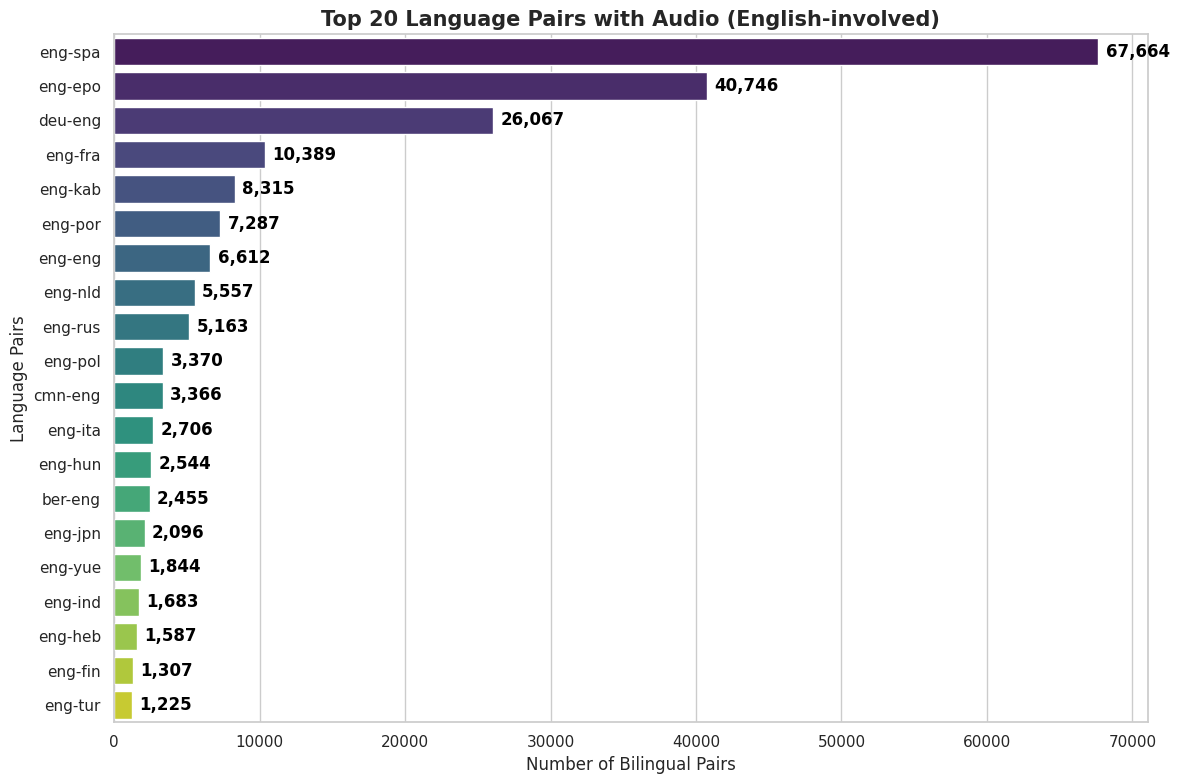
\includegraphics[width=\linewidth]{images/tatoeba_data.png}
%                 \caption{\footnotesize Parallel sentence pairs from Tatoeba for multilingual evaluation.}
%                 \label{fig:tatoeba}
%             \end{figure}
%         \end{column}
%
%         \begin{column}{0.55\textwidth}
%             \textbf{Source 2: YouTube Multilingual Audio}
%             \begin{itemize}
%                 \item \textbf{Sources:} MrBeast, Mark Rober, NatGeo, Nick DiGiovanni, Jamie Oliver.
%                 \item \textbf{Processing:} Audio-to-Audio chunking ($10$--$30$\,s segments) or VAD-based pause-splitting.
%                 \item \textbf{High-Volume Corpus:} Thousands of videos, thousands of hours of high-fidelity speech.
%                 \item \textbf{Multilingual Parallelism:} Content in \textbf{40+ languages}, offering aligned corpus for S2S training.
%             \end{itemize}
%         \end{column}
%     \end{columns}
%
%     \vfill
%     \begin{figure}
%         \centering
%         
\includegraphics[width=0.7\linewidth]{images/VNlaw.png}
%         \caption{\footnotesize Vietnamese IP Law amendment 131/2025/QH15 (effective 01/4/2026).}
%         \label{VN_law}
%     \end{figure}
% \end{frame}

\begin{frame}[t]{Data Sources}
    \begin{columns}[T,onlytextwidth]
        \begin{column}{0.42\textwidth}
            \textbf{Source 1: Tatoeba}
            \begin{figure}
                \centering
                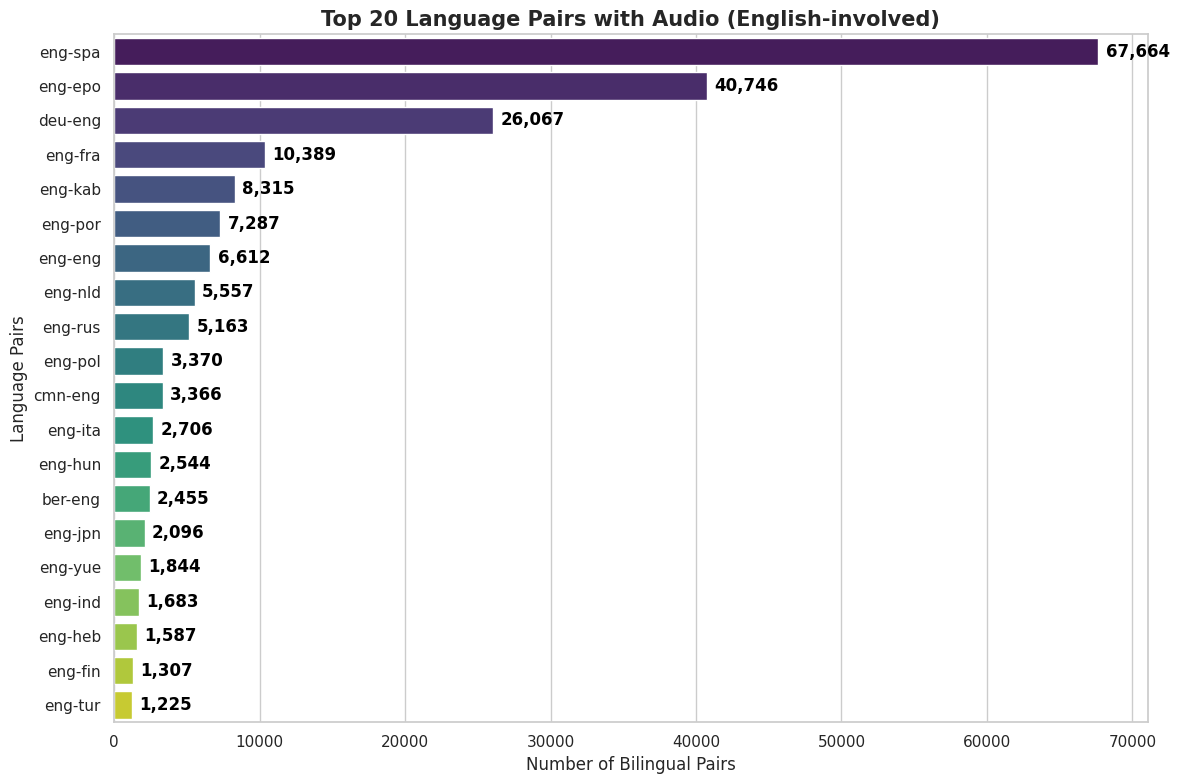
\includegraphics[width=\linewidth]{images/tatoeba_data.png}
            \end{figure}
            {\footnotesize Parallel sentence pairs for multilingual evaluation.}
        \end{column}

        \begin{column}{0.56\textwidth}
            \textbf{Source 2: YouTube Multilingual Audio}
            \begin{itemize}
                \item \textbf{Sources:} MrBeast, Mark Rober, NatGeo, Nick DiGiovanni, Jamie Oliver.
                \item \textbf{Processing:} 10--30s chunking or VAD-based pause splitting.
                \item \textbf{High-volume corpus:} Thousands of videos and hours of high-fidelity speech.
                \item \textbf{Multilingual parallelism:} Content in 40+ languages for aligned S2S training.
            \end{itemize}
        \end{column}
    \end{columns}
\end{frame}

\begin{frame}[t]{Legal \& Licensing Considerations}
    \begin{columns}[T,onlytextwidth]
        \begin{column}{0.48\textwidth}
            \begin{itemize}
                \item Public online audio does not automatically imply free reuse for model training.
                \item The project must consider copyright, licensing, and fair-use limitations.
                \item For a production system, data sourcing should prioritize public, licensed, synthetic, or explicitly permitted datasets.
            \end{itemize}
        \end{column}

        \begin{column}{0.5\textwidth}
            \begin{figure}
                \centering
                
\includegraphics[width=\linewidth]{images/VNlaw.png}
            \end{figure}
            {\footnotesize Vietnamese IP law amendment relevant to data reuse.}
        \end{column}
    \end{columns}
\end{frame}


% ============================================================
% Slide 6: Model Selection & Optimization (1/2)
% ============================================================
\begin{frame}{Model Selection: SeamlessM4T}
    \begin{block}{Why SeamlessM4T?}
        A single unified model that supports \textbf{all four translation modes} --- T2T, S2T, T2S, S2S --- across 100+ languages, eliminating the need for separate ASR + MT + TTS pipelines.
    \end{block}

    \pause

    \begin{table}[]
        \footnotesize
        \begin{tabular}{@{}llll@{}}
        \toprule
        \textbf{Model} & \textbf{Size} & \textbf{CPU MBP M1 T2T} & \textbf{GPU T4 T2T} \\ \midrule
        \texttt{seamless-m4t-medium} & $\sim$6.4\,GB & 3--15\,s & $<$ 1\,s \\
        \texttt{seamless-m4t-large}  & $\sim$10.7\,GB & 20--25\,s & 1--3\,s \\
        \bottomrule
        \end{tabular}
        \caption{\footnotesize Warm inference latency comparison (text-to-text).}
    \end{table}

    \vspace{4pt}
    \textbf{Trade-off:} We chose \textbf{medium} for demo practicality --- loads faster, fits in 8\,GB RAM, and still delivers strong translation quality across our 12 supported languages.
\end{frame}


% ============================================================
% Slide 7: Model Selection & Optimization (2/2)
% ============================================================
\begin{frame}[t]{Inference Optimization}
\small

\textbf{Problem:} Na\"ive integration caused 30--60 s cold starts and
redundant computation per request.

\vspace{4pt}
\textbf{Optimizations applied:}
\begin{enumerate}\setlength{\itemsep}{3pt}
    \item \textbf{Eager loading:} load model in the background at server startup.
    \item \textbf{--noreload:} prevent Django autoreload from restarting the process.
    \item \textbf{Single bundle fetch:} retrieve model + processor once per request.
    \item \textbf{Pre-prepared audio:} preprocess once and reuse across steps.
    \item \textbf{Conditional \texttt{gc.collect()}:} run only on CUDA, skip on CPU.
\end{enumerate}

\vspace{4pt}
\textbf{Result:} Warm text-to-text inference reaches \textbf{1--5 s} on CPU
after a one-time \textbf{15--30 s} cold start.
\end{frame}


% ============================================================
% Slide 8: Deployment Overview
% ============================================================
\begin{frame}{System Architecture \& Deployment}
    \centering
    \resizebox{0.92\textwidth}{!}{%
    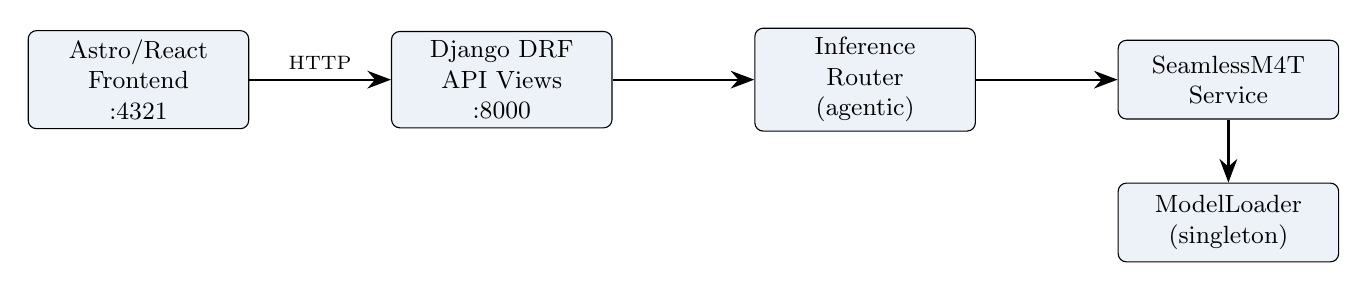
\begin{tikzpicture}[
        node distance=8mm and 18mm,
        every node/.style={align=center, font=\small},
        box/.style={draw, rounded corners=3pt, minimum width=28mm, minimum height=10mm, fill=HCMUSBlue!8},
        arrow/.style={thick, -{Stealth[length=3mm]}}
    ]
        \node[box] (fe) {Astro/React\\Frontend\\:4321};
        \node[box, right=of fe] (api) {Django DRF\\API Views\\:8000};
        \node[box, right=of api] (router) {Inference\\Router\\(agentic)};
        \node[box, right=of router] (svc) {SeamlessM4T\\Service};
        \node[box, below=of svc] (ml) {ModelLoader\\(singleton)};

        \draw[arrow] (fe) -- node[above]{\scriptsize HTTP} (api);
        \draw[arrow] (api) -- (router);
        \draw[arrow] (router) -- (svc);
        \draw[arrow] (svc) -- (ml);
    \end{tikzpicture}
    }

    \vspace{10pt}

    \begin{columns}[t]
        \begin{column}{0.5\textwidth}
            \textbf{Four Translation Modes}
            \begin{itemize}
                \item Text $\to$ Text
                \item Speech $\to$ Text
                \item Text $\to$ Speech
                \item Speech $\to$ Speech
            \end{itemize}
        \end{column}
        \begin{column}{0.5\textwidth}
            \textbf{Deployment Options}
            \begin{itemize}
                \item \texttt{make dev} (local)
                \item Docker Compose
                \item GPU server (CUDA)
            \end{itemize}
        \end{column}
    \end{columns}
\end{frame}


% ============================================================
% Slide 9: Agentic AI Component
% ============================================================
\begin{frame}[t]{Agentic AI Component: Intent-Driven Orchestration}
\small

\begin{block}{The Role of the Agent}
Instead of a passive pipeline, the Agent acts as a \textbf{Decision Engine}
that orchestrates translation based on user intent and environmental context.
\end{block}

\vspace{2pt}
\textbf{Core Agentic Behaviors:}
\begin{itemize}\setlength{\itemsep}{4pt}
    \item \textbf{Autonomous Context Routing:}
    Detect target language and situational context
    (e.g., dining, emergency, directions).

    \item \textbf{Proactive Suggestion Engine:}
    Suggest culturally appropriate opening phrases
    from recognized intent (e.g., ``I'm lost'').
\end{itemize}

\vspace{2pt}
\begin{block}{Backend Implementation}
\texttt{InferenceRouter} checks model readiness, language support,
audio duration, and memory pressure before inference.
\end{block}

\end{frame}


% ============================================================
% Slide 10: Continual Learning & Monitoring
% ============================================================
% \begin{frame}{Continual Learning \& Monitoring Strategy}
%     \begin{block}{The Feedback Loop}
%         \small
%         \begin{enumerate}
%             \item \textbf{Collect \& Filter:} Directly pool samples rated as \textbf{``Good''} by users for high-quality SFT data.
%             \item \textbf{Data Refinement:} For \textbf{``Bad''} samples, Admins use:
%                 \begin{itemize}
%                     \scriptsize
%                     \item \textbf{Large Models:} To regenerate correct audio/text for large-scale batches.
%                     \item \textbf{Manual Collection:} For niche or high-priority failure cases.
%                 \end{itemize}
%             \item \textbf{Evolve:} Apply \textbf{LoRA Fine-tuning} on the merged high-quality dataset.
%             \item \textbf{Deploy:} A/B testing against baseline before full production release.
%         \end{enumerate}
%     \end{block}
%
%     \vspace{6pt}
%     \textbf{Monitoring endpoints:}
%     \begin{itemize}
%         \item \texttt{/api/health/} --- full system diagnostics (model status, device, memory, timing)
%         \item \texttt{/api/readiness/} --- lightweight 200/503 probe for automation
%         \item Per-request \texttt{timing} field --- preprocess, transcript, translation latency breakdown
%     \end{itemize}
% \end{frame}

\begin{frame}[t]{Continual Learning Strategy}
\small

\begin{block}{The Feedback Loop}
\begin{enumerate}\setlength{\itemsep}{4pt}
    \item \textbf{Collect \& Filter:}
    Pool samples rated as \textbf{``Good''} for high-quality SFT data.

    \item \textbf{Refine ``Bad'' cases:}
    \begin{itemize}\setlength{\itemsep}{2pt}
        \item \textbf{Large models:} regenerate corrected audio/text at scale.
        \item \textbf{Manual collection:} handle niche or high-priority failures.
    \end{itemize}

    \item \textbf{Evolve:}
    Apply \textbf{LoRA fine-tuning} on the merged high-quality dataset.

    \item \textbf{Deploy:}
    Run \textbf{A/B testing} against the baseline before release.
\end{enumerate}
\end{block}

\end{frame}

\begin{frame}[t]{Monitoring Strategy}
\small

\textbf{Monitoring endpoints:}
\begin{itemize}\setlength{\itemsep}{5pt}
    \item \texttt{/api/health/} --- full diagnostics:
    model status, device, memory, timing.

    \item \texttt{/api/readiness/} --- lightweight 200/503 probe
    for automation and deployment checks.

    \item Per-request \texttt{timing} field --- latency breakdown for
    preprocessing, transcript generation, and translation.
\end{itemize}

\vspace{6pt}
\begin{block}{Operational Goal}
Detect failures early, track latency drift, and support safer model updates
over time.
\end{block}

\end{frame}


% ============================================================
% Slide 11: Data Privacy & Model Robustness
% ============================================================
\begin{frame}{Data Privacy \& Model Robustness}
    \begin{columns}[t]
        \begin{column}{0.50\textwidth}
            \textbf{Privacy by Design}
            \begin{itemize}
                \item Audio processed in-memory; temp files deleted after each request.
                \item No persistent storage of user audio beyond generated output.
                \item Model runs \textbf{entirely on-device} --- zero third-party API calls.
                \item All inputs validated at API boundary (serializers + router).
            \end{itemize}
        \end{column}

        \pause

        \begin{column}{0.50\textwidth}
            \textbf{Robustness Strategy}
            \begin{itemize}
                \item \textbf{English as Pivot:} For weak language pairs (e.g., Vie--Jpn), bridge via English to leverage high-density semantic embeddings.
                \item \textbf{Confidence Thresholds:} Fallback to ``Clarification Mode'' if pivot uncertainty is high.
                \item \textbf{Input Guards:} Audio duration limit (120\,s), file size limit (25\,MB), extension validation.
            \end{itemize}
        \end{column}
    \end{columns}
\end{frame}


% ============================================================
% Slide 12: Ethics, Privacy & Risks
% ============================================================
% \begin{frame}{Ethics \& Fairness: Responsible AI Framework}
%     \begin{columns}[t]
%         \begin{column}{0.50\textwidth}
%             \textbf{Ethics Impact Statement}
%             \begin{itemize}
%                 \item \textbf{Beneficiaries:} International travelers (reducing friction) and local businesses (increasing accessibility).
%                 \item \textbf{Potential Harm:} Users with strong regional accents or speech impairments might face exclusion if the model is not robust.
%             \end{itemize}
%
%             \vspace{4pt}
%             \textbf{Bias \& Fairness Risks}
%             \begin{itemize}
%                 \item \textbf{Language Bias:} Performance gap between high-resource (English) and low-resource languages (Vietnamese).
%                 \item \textbf{Accent Bias:} Potential inaccuracy for Northern vs.\ Southern Vietnamese dialects.
%             \end{itemize}
%         \end{column}
%
%         \pause
%
%         \begin{column}{0.50\textwidth}
%             \begin{block}{Mitigation Strategies}
%                 \small
%                 \textbf{1. PII Anonymization:}
%                 \begin{itemize}
%                     \scriptsize
%                     \item Scrubbing PII from audio before any Admin/Model review.
%                 \end{itemize}
%
%                 \textbf{2. Diverse Training Data:}
%                 \begin{itemize}
%                     \scriptsize
%                     \item YouTube multilingual corpus covers varied accents and speaking styles.
%                 \end{itemize}
%
%                 \textbf{3. Evaluation Protocol:}
%                 \begin{itemize}
%                     \scriptsize
%                     \item BLASER + MOS scoring across all 12 supported language pairs.
%                     \item Per-language performance tracking to detect degradation.
%                 \end{itemize}
%             \end{block}
%         \end{column}
%     \end{columns}
% \end{frame}

\begin{frame}[t]{Ethics \& Fairness: Responsible AI Framework}
\small

\begin{columns}[T,onlytextwidth]
    \begin{column}{0.48\textwidth}
        \textbf{Ethics Impact Statement}
        \begin{itemize}\setlength{\itemsep}{4pt}
            \item \textbf{Beneficiaries:} International travelers and local businesses.
            \item \textbf{Potential Harm:} Users with strong regional accents or speech impairments may face exclusion if the model is not robust.
        \end{itemize}
    \end{column}

    \begin{column}{0.48\textwidth}
        \textbf{Bias \& Fairness Risks}
        \begin{itemize}\setlength{\itemsep}{4pt}
            \item \textbf{Language Bias:} Performance gaps between high-resource and low-resource languages.
            \item \textbf{Accent Bias:} Potential inaccuracy across Vietnamese regional dialects.
        \end{itemize}
    \end{column}
\end{columns}

\end{frame}

\begin{frame}[t]{Mitigation Strategies}
\small

\begin{block}{Responsible AI Mitigation}
\begin{enumerate}\setlength{\itemsep}{5pt}
    \item \textbf{PII Anonymization:}
    Scrub personal information from audio before any admin or model review.

    \item \textbf{Diverse Training Data:}
    Use multilingual speech data with broader accent and speaking-style coverage.

    \item \textbf{Evaluation Protocol:}
    Track BLASER, MOS, and per-language performance to detect degradation early.
\end{enumerate}
\end{block}

\end{frame}


% ============================================================
% Slide 13: Future Work & Conclusion
% ============================================================
% \begin{frame}{Future Work \& Conclusion}
%     \textbf{Current Limitations}
%     \begin{itemize}
%         \item Turn-based translation (2--15\,s per utterance on CPU) --- not live streaming.
%         \item Frontend language list maintained separately from backend config.
%         \item Generated audio served via Django debug mode; production needs object storage.
%     \end{itemize}
%
%     \pause
%     \vspace{6pt}
%
%     \textbf{Planned Improvements}
%     \begin{itemize}
%         \item \textbf{WebSocket streaming} for progressive output delivery.
%         \item \textbf{INT8 quantization} for faster CPU inference.
%         \item \textbf{Speaker diarization} for multi-participant scenarios.
%         \item \textbf{Audio chunking} to handle inputs beyond the 120\,s cap.
%         \item \textbf{Multi-session support} for concurrent translations.
%     \end{itemize}
%
%     \vspace{8pt}
%     \begin{block}{Honest Positioning}
%         This system is a \textbf{near-real-time, turn-based travel translation assistant} --- practical for asynchronous interactions where participants take turns speaking. After warmup, each utterance translates in 2--15\,s (CPU) or under 3\,s (GPU).
%     \end{block}
% \end{frame}

\begin{frame}[t]{Current Limitations}
\small

\textbf{Current Limitations}
\begin{itemize}\setlength{\itemsep}{4pt}
    \item Turn-based translation (\textbf{2--15 s} per utterance on CPU), not live streaming.
    \item Frontend language list is maintained separately from backend config.
    \item Generated audio is served via Django debug mode; production needs object storage.
\end{itemize}

\vspace{6pt}
\begin{block}{Honest Positioning}
This system is a \textbf{near-real-time, turn-based travel translation assistant}.
It is practical for asynchronous interactions where speakers take turns.
After warmup, each utterance translates in \textbf{2--15 s} on CPU or under
\textbf{3 s} on GPU.
\end{block}

\end{frame}

\begin{frame}[t]{Future Work}
\small

\textbf{Planned Improvements}
\begin{itemize}\setlength{\itemsep}{5pt}
    \item \textbf{WebSocket streaming} for progressive output delivery.
    \item \textbf{INT8 quantization} for faster CPU inference.
    \item \textbf{Speaker diarization} for multi-participant scenarios.
    \item \textbf{Audio chunking} for inputs beyond the 120 s cap.
    \item \textbf{Multi-session support} for concurrent translations.
\end{itemize}

\vspace{6pt}
\begin{block}{Longer-Term Direction}
Move from turn-based translation toward more responsive, scalable, and
multi-user speech translation in realistic travel settings.
\end{block}

\end{frame}

\end{document}
